\documentclass[conference,compsoc]{IEEEtran}

% This is because IEEE is a bad latex style
\newtheorem{definition}{Definition}
\newtheorem{lemma}{Lemma}
\newtheorem{proof}{Proof}
% \documentclass[sigconf, anonymous]{acmart}

% \usepackage{usenix-2020-09}



\usepackage{enumitem}
\usepackage{arydshln}
% \usepackage{amsthm}
\usepackage{amssymb}
\usepackage{subcaption}
% \usepackage{subfig}
\usepackage{subcaption}
\usepackage{graphicx}
\usepackage{amsmath}
\usepackage{url}
\usepackage{color}
\usepackage{booktabs}
\usepackage{multirow}
\usepackage{algorithm}
\usepackage{algpseudocode, float}
\usepackage{bbding}
\usepackage{bbding}
\usepackage{tikz}
\usetikzlibrary{shapes.geometric,arrows,decorations.markings, arrows.meta}
\usetikzlibrary{positioning, calc}


\usepackage{forest}

\usetikzlibrary{graphs}
\usetikzlibrary{arrows,automata}

\forestset{%
angle below/.style={
tikz+={%
\draw ($(!1.child anchor)!.25!(.parent anchor)$) [bend right=15] to ($(.parent anchor)!.75!(!l.child anchor)$);
},
},
small angle below/.style={
tikz+={%
\draw ($(!1.child anchor)!.5!(.parent anchor)$) [bend right=15] to ($(.parent anchor)!.5!(!l.child anchor)$);
},
},
arrow below/.style={
tikz+={%
\draw[->] ($(!1.child anchor)!.30!(.parent anchor)$) [bend right=20] to ($(.parent anchor)!.7!(!l.child anchor)$);
},
},
}




% \raggedbottom
% 
\pagestyle{plain}
\begin{document}


\title{Attack Tree Distance: a practical examination of tree difference measurement within cyber security}

\iffalse{
    \author{Nathan D. Schiele}
    \orcid{0000-0003-1186-1503}
    \affiliation{\institution{Leiden University}
        \city{Leiden}
        \country{The Netherlands}}
    \email{n.d.schiele@liacs.leidenuniv.nl}


    \author{Olga Gadyatskaya}
    \orcid{0000-0002-3760-9165}
    \affiliation{\institution{Leiden University}
        \city{Leiden}
        \country{The Netherlands}}
    \email{o.gadyatskaya@liacs.leidenuniv.nl}
}\fi
\author{Anonymized for submission}




% \acmConference[ACSAC]{ACSAC}
% \acmYear{2024}
% \acmBooktitle{Proceedings of the 32nd ACM Symposium on the Foundations of Software Engineering (FSE '24), November 15--19, 2024, Porto de Galinhas, Brazil}
% \acmBooktitle{Submission to ACSAC'24}

% \settopmatter{printfolios=true}

% \begin{teaserfigure}
%     \includegraphics[width=\textwidth]{img/Teaser02}
%     \caption{Participant created ADT}
%     \Description{A collage of ADTs that were created by participants}
%     \end{teaserfigure}

% \begin{teaserfigure}
% \includegraphics[width=\textwidth]{img/CollageTeaser}
% \caption{Assorted participant created ADTs}
% \Description{A collage of ADTs that were created by participants}
% \end{teaserfigure}




\maketitle              % typeset the header of the contribution
\newcommand{\OG}[1]{{\color{blue} OG: #1}}
\newcommand{\NS}[1]{{\color{purple} NS: #1}}

\newcommand{\etal}{et al.}
\newcommand{\id}[2]{#1-#2}
\newcommand{\hypothesis}[1]{$\text{H}_\text{#1}$}
\newcommand{\RQ}[1]{\textbf{RQ#1}}

\newcommand{\ICS}{NCS}
\newcommand{\SEC}{CS}

\newcommand{\AND}{AND}
\newcommand{\SAND}{SAND}
\newcommand{\OR}    {OR}



\newcommand{\hypoCheckUnderstand}   {1}
\newcommand{\hypoSecondADT}         {2}
\newcommand{\hypoErrorAmount}       {3}
\newcommand{\hypoSelfUnderstand}    {4}
\newcommand{\hypoCommunicationTool} {5}
\newcommand{\hypoAnalysisTool}      {6}
\newcommand{\hypoWrittenComparison} {7}
\newcommand{\hypoIntentionToUse}    {8}
\newcommand{\hypoThirdADT}          {9}


\newcommand{\hypoMultipleParent}  {3-1}
\newcommand{\hypoMultipleRefinement}  {3-2}
\newcommand{\hypoMulipleCountermeasure}  {3-3}
\newcommand{\hypoSingleChildNodes}  {3-4}

\newcommand{\hypoGrades}            {10 - Not used}


\newcommand{\hResponse}[1]{\texttt{#1} - }

\newcommand{\anonfoot}{\footnote{Anonymized for submission}}


\newcommand{\qIndent}{4em}
\newcommand{\qsIndent}{2em}
\newcommand{\surveyq}[1]{\textbf{#1:}}





\begin{abstract}
    \absSection{Context} Attack trees are a recommended threat modeling tool, but there is no established method to compare them.
\absSection{Objective} We aim to compare varied distance metrics which are capable of comparing ``real'' attack trees, based on both the structure of the tree itself and the meaning of the node labels.
    \absSection{Method} We define four methods of comparison (three novel and one established) and compare them to a dataset of attack trees created from a study run on students ($n=39$). These attack trees all follow from the same scenario, but have slightly different labels.
\absSection{Results} We show a repeatable method of experimental validation. From this, we find that applying semantic similarity as a means of comparing node labels is a valid approach. Further, we find that tree edit distance (established) and radical distance (novel) are the most promising methods of comparison in most circumstances.
    \absSection{Conclusion} We show that these two methods are valid as means of comparing attack trees, and suggest a novel technique for using semantic similarity to compare node labels. We further suggest that these methods can be used to compare attack trees in a real-world scenario, and that they can be used to identify similar attack trees.
\end{abstract}



\section{Background}
\label{sec:background}


\begin{figure*}
    \includegraphics[width=\linewidth]{img/TargetAT.png}
    \caption{An attack tree adapted from Naik \etal~\cite{naikEvaluationPotentialAttack2022} that is used in the study described in Section~\ref{sec:methodology}. }
    \label{fig:tartgetAT}
\end{figure*}

We define attack trees, as initially described by Bruce Schneier~\cite{schneierAttackTrees1999}, to be a rooted acyclic structure with the following recursive definition adapted from Gadyatskaya~\etal~\cite{gadyatskayaRefinementAwareGenerationAttack2017}.

\begin{definition} \label{def:attack-tree} An attack tree  is defined as $T = \ATnode{1}{1}\Delta(\ATnode{2}{1},...,\ATnode{2}{i})$. Where $\ATnode{d}{i} = \ATlabel{d}{i}\Delta(\ATnode{d+1}{j},...,\ATnode{d+1}{k})$

    % We define the $i\text{th}$ node according to left-right post-order number to be the following, $T[i] = b\Delta(T[j],...,T[k])$. 

    % We give $b$ to be some action within the attack scenario, which is the node label of $t$. For clarity, we additionally refer to this label as $t.\text{label}$. We give $\Delta$ to be the refinement $\Delta = \AND|\OR|\SAND$. For clarity and consistency, we refer to the refinement of a given node to be $t.\Delta$. Following the refinement, we have a list of nodes which are the children of $t$, defined as $t_0,...,t_i$ which is the left to right order of the children (regardless of if order is significant). We refer to the list of children as $t.\text{children}$. This list of nodes can be empty, in the case of leaf nodes.

    % For clarity and consistency, we refer to the refinement of a given node to be $t.\Delta$. Following the refinement, we have a list of nodes which are the children of $\ATnode{d}{i}$, defined as $\ATnode{d+1}{j},...,\ATnode{d+1}{k}$ where $j \ge 1$ and $k \ge j$, which is the left to right order of the children (regardless of if order is significant). We refer to the list of children as $\ATnode{d}{i}.\text{children}$. This list of nodes can be empty, in the case of leaf nodes.

    Each node within an attack tree is a sub-tree unto itself. We define each node as $\ATnode{d}{i}$ where $d$ is the depth of the node (distance from the root, given the root has a starting distance of 1), and $i$ is the number of that node counting from the left most node at depth $d$ (starting from 1). We define a mapping of each node to a label space, where the label of node $\ATnode{d}{i}$ is given as $\ATlabel{d}{i}$. We give $\Delta$ to be the refinement $\Delta = \AND|\OR$. We further define the following functions to retrieve associated information of some node $\ATnode{d+1}{j}$. We define the $\Delta(\ATnode{d}{i})$ function to return the refinement of a given node. We define the child function, $\childFunc{\ATnode{d}{i}}$ to return a list of nodes which are the children of a given node, defined as $\ATnode{d+1}{j},...,\ATnode{d+1}{k}$ where $j \ge 1$ and $k \ge j$, which is the left to right order of the children (regardless of if order is significant). This list of nodes can be empty, in the case of leaf nodes. Finally, we define the parent function, $\parentFunc{\ATnode{d}{i}}$ to return the parent of a given node.
\end{definition}


\section{Research}

Our primary research goal is to determine a mechanism to calculate the distance between two attack trees. This is a novel problem, as attack trees contain the concept of refinements, and the application of tree edit distance to the cybersecurity domain has yet to be seen.

\subsection{Research Questions}

We posit the following research questions:

\begin{enumerate}
    \item[\RQ{1}] How can we best calculate the distance between two attack trees?
    \item[\RQ{2}] Is this method of attack tree distance valid?
    \item[\RQ{3}] What are the industry applications of attack tree distance?
\end{enumerate}


% \subsection{Requirements}
% \label{ssec:requirements}

% The application of tree edit distance to attack trees requires a number of considerations. These considerations are as follows:


% \subsubsection{Refinement Awareness}
% \label{sssec:refinement}

% The primary difference between attack trees and most directed acyclic graphs (DAGs) are the presence of refinements, or the given relationship between children. This is a critical part of the attack tree structure and must be included in the tree edit distance algorithm.

% \subsubsection{Semantic Label Similarity}
% \label{sssec:label-similarity}

% In early iterations of tree edit distance problems, node labels were said to be equivalent if the labels were identical. However, in most contexts, it will not be the case that node labels will be identical. Especially in the context of cyber security, it is easily possible for two nodes in a DAG to represent the same idea but presented in a radically different manner. As such, the distance between attack trees must have a mechanism to account for the similarity between node labels on the basis of their meaning.

% \subsubsection{Order of children}
% \label{sssec:order-of-children}

% It is a known problem that tree edit distance of unordered trees is an \textit{NP}-Complete problem~\cite{zhang_editing_1992}. However, attack trees are unique in that the order of children is dependent on the refinement of the parent node. As such, the distance between attack trees must be able to account for the order of children in the context of the refinement of the parent node. In the case of \AND\ and \OR\ refinements, the children are unordered. However, in the case of \SAND\ (\emph{Sequential} \AND) refinements, the order of children is important. As such, the edit distance between two attack trees must optimize to allow for the reordering of nodes when calculating the edit distance; however, this optimization must be such that it is selectively applicable, and can be not applied in the case of \SAND\ refinements.

% \subsubsection{Metric}
% \label{sssec:metric}

% The distance between two attack trees must be a metric. That is to say, the distance between two attack trees must be non-negative, symmetric, and satisfy the triangle inequality.



% \subsubsection{Consensus Trees}
% \label{sssec:consensus-trees}

% \NS{I dunno if this should be included in this paper - but it'd make it SO MUCH EASIER to argue utility}


% One potential utility of tree edit distance would be to allow for the recognition missing vectors or components of attack trees \NS{cite AG distance paper}. For example, if we find that one tree is a whole subset of another tree, that is the consensus tree between two trees is equivalent to one of the trees, then we can infer that the components of the larger tree are components that would be directly applicable to the subset tree. As such, we can use this method of calculating a consensus tree to find missing components of attack trees.

\section{Background}

Distance between data structures is not a new concept. Many works have explored the idea of ``distance'' between strings. In string edit distance, where the difference in strings is given my a min-cost path taken by either adding a character, removing a character or replacing a character. By fining the minimum cost needed to transform one string into another, a ``distance'' value can be given. As the higher cost a transformation, the further apart two strings must be \NS{cite all the string edit distance papers}.

Much of the work in this field has built upon work by Kuo-Chung Tai who suggested that the distance between trees is similar to several previous works comparing the differences in strings~\cite{tai_tree--tree_nodate}.

\section{Related Work}

Tree Edit Distance is not a new computational challenge. However, most of the development on tree edit distance focuses calculation optimization. As shown by Zhang~\etal, the tree edit distance problem for unordered trees is an \textit{NP}-Complete problem~\cite{zhang_editing_1992}. As such, the develop of novel optimal calculation strategies is necessary to enable comparison of larger tree structures. Zhang and Shasha proposed a commonly cited simple algorithm for calculating tree edit distance~\cite{zhang_simple_1989}. We use this algorithm in this paper as it is a common strategy for implementing and testing extensions to tree edit distance. As such, optimizations based on the Zhang and Shasha algorithm can be applied to our methodology as we show in section \NS{When I write that section, I'll reference it here}.

Tree edit distance, like string edit distance, has a wide array of applications. Just as string edit distance has been used to compare sequences of DNA \NS{cite},

\section{Validation}
\label{sec:validation}

In order to evaluate any approach for comparing attack trees, we must first establish a means of validating the results and assessing the quality of this approach. We propose two methods of validating the distance measures:

\textbf{Theoretical validation}. This validation method involves defining a series of basic transformation examples (BTEs) that represent the most fundamental ways in which two attack trees could differ from each other. These BTEs can be adapted to only express the transformations that we would expect to see, or that we explicitly would desire to compare two distance measures along. For example, if we only wish to evaluate distance measures according to their ability to compare leaf nodes (as the traditional attack tree semantics expect~\cite{mauwFoundationsAttackTrees2006}), we could define a set of BTEs which only shows changes in leaf nodes. For a more comprehensive comparison, we can define a larger set of BTEs to show all possible basic transformations. This is what we do in Section~\ref{sec:methodology}. We argue that if any transformation can be expressed as a series of BTEs, then we can validate the distance measure by comparing the distance measure's output to the expected distance of each BTE.

\textbf{Experimental validation}. We offer an experimental design that can be used to validate a distance measure on ``real-world'', human-produced data. This requires a dataset that contains two sets of attack tree models. First, we require a base set of trees which should all be identical. This can be created by asking participants to create an attack tree describing the same precisely defined scneario. Any variation between the trees would likewise be representative of ``real-world'' label variation, and not due to differences in attack steps identified by distinct experts. In this way, we can evaluate how the distance measures handle similar but not fully identical data. 

Second, we require the base set of trees to be slightly expanded by the authors. This results in a second set of trees that are expected to be slightly different, but not very diverse. At the same time, the base set contains attack trees that are subtrees of this second set. This allows us to evaluate the behavior of the distance measures when comparing a tree to a known subset of that tree, and to compare a set of attack trees that are slightly different from each other. This behavior should be predictable, and we can access distance measures if they display the behavior we expect. We describe the details of our study design and the data collection process in Section~\ref{sec:methodology}.
\section{Semantic Similarity}
\label{sec:semantic-similarity}


\tikzstyle{block} = [rectangle, draw, fill=black!290,
text width=5em, text=white,  text centered, rounded corners, minimum height=4em]
\begin{figure*}
    \centering
    \begin{tikzpicture}[node distance = 2cm, auto]
        % Place nodes
        \node [xshift=-5cm](t1) {$\ATlabel{d}{i}$};
        \node [below of = t1] (t2) {$\ATlabel{e}{j}$};
        \node [block, below right = .5cm and 1cm of t1, yshift=.3cm]  (genbeddings) {\shortstack{Generate\\Semantic\\Embeddings}};
        \node [right of = t1, xshift=4cm]  (et1) {$\vec{e}(\ATlabel{d}{i})$};
        \node [below of = et1]  (et2) {$\vec{e}(\ATlabel{e}{j})$};
        \node [block, right of = genbeddings, xshift= 4.5cm]  (comp) {\shortstack{Vector\\Comparison}};
        \node [right of = comp, xshift = 2cm]  (end) {$\delta(\ATlabel{d}{i}, \ATlabel{e}{j})$};


        % Draw edges
        \draw [->] (t1.east)  -| ($(t1)!0.5!(genbeddings)$) coordinate |-(genbeddings);
        \draw [->] (t2.east)  -| ($(t2)!0.5!(genbeddings)$) coordinate |-(genbeddings);
        \draw [->] (genbeddings.east)  -| ($(genbeddings)!0.5!(et1)$) coordinate |-(et1);
        \draw [->] (genbeddings.east)  -| ($(genbeddings)!0.5!(et2)$) coordinate |-(et2);
        \draw [->] (et1.east)  -| ($(et1)!0.5!(comp)$) coordinate |-(comp);
        \draw [->] (et2.east)  -| ($(et2)!0.5!(comp)$) coordinate |-(comp);
        \draw [->] (comp)  -- (end);
    \end{tikzpicture}
    \caption{Process of calculating the distance between two node labels.}
    \label{fig:semanticreplacement}
\end{figure*}

In most of the tree distance measures described in Section~\ref{sec:related-work}, nodes are only matched, or considered equivalent, if the node labels are identical. Taking one example from our experiment (described in Sections~\ref{sec:methodology}~and~\ref{sec:results}), this would result in the node labels ``Obtain personal data'' and ``obtain personal data'' to not be matched, as these labels are not identical. While other label reconciliation schemes have been proposed, many are based on the string edit distance (Levenshtein distance) of the two node labels. This method is not ideal as it can result in two nodes that are entirely unrelated but with similar vocabulary having small edit distances, while two nodes that are related or identical having large edit distances. In Table~\ref{tab:distances}, we provide a few examples of potential node label comparisons using both normalized Levenshtein distance and semantic similarity. Semantic similarity is calculated using the BERT method and is shown graphically in Figure~\ref{fig:semanticreplacement}. The normalized Levenshtein distance is calculated as one minus the Levenshtein distance divided by the length of the longest string:

\[
\delta\left(\ATlabel{d}{i}, \ATlabel{e}{j}\right) = 1 - \frac{\text{Levenshtein}\left(\ATlabel{d}{i}, \ATlabel{e}{j}\right)}{\max\left(\left|\ATlabel{d}{i}\right|, \left|\ATlabel{e}{j}\right|\right)}
\]

% \[
% \delta(b_i, b_j) = 1 - \frac{\text{Levenshtein}(b_i, b_j)}{\max(|b_i|, |b_j|) }
% \]


In Table~\ref{tab:distances}, can see the extreme example of ``door open'' and ``open door'' which has a Levenshtein distance of 8 (normalized Levenshtein distance of 0), as all letters must be changed. However, the semantic similarity is 0.992, which is the highest of our selected examples. This is because the two labels are near identical in meaning, and the only difference is the order of the words. In contrast, the two labels ``obtain personal data'' and ``obtain personnel'' have a normalized Levenshtein distance of .5882, but a semantic similarity of 0.4507. This is because the two labels are not related, but due to similar language, the normalized string edit distance is relatively small. If we implemented a distance between the two labels
$\delta\left(\ATlabel{d}{i}, \ATlabel{e}{j}\right)$ %$\delta\left(\ATlabel{d}{i}, \ATlabel{e}{j}\right)$ 
to be based on Levenshtein distance, nodes that should incur a cost to edit may not while those that should not incur a cost to edit may.
% This method is not ideal, as it is possible for two unrelated nodes to have small edit distances, such as ``obtain personnel'' and ``obtain personal data'' (edit distance of 7) while related nodes have larger edit distances; such as comparing ``obtain personal data'' and ``gather private info'' (edit distance of 15). In our first example, the two nodes are not related, but due to similar verbiage, the edit distance is relatively small. In the second example, the two nodes have identical meaning, but due to different vocabulary used, the Levenshtein distance between them is significantly larger. If we implemented a distance between the two labels  $\delta\left(\ATlabel{d}{i}, \ATlabel{e}{j}\right)$ to be based on Levenshtein distance, nodes that should incur a cost to edit may not while those that should not incur a cost to edit may.

\begin{table}[]
    \begin{tabular}{@{}llll@{}}
        \toprule
        Label 1              & Label 2             & \begin{tabular}[c]{@{}l@{}}Normalized\\Levenshtein\\ Distance\end{tabular} & \begin{tabular}[c]{@{}l@{}}Semantic \\ Similarity\end{tabular} \\ \midrule
        obtain personal data & obtain personnel    & 0.5882                                                                     & 0.4507                                                         \\
        obtain personal data & gather private info & 0.1176                                                                     & 0.5521                                                         \\
        break open safe      & break open door     & 0.6923                                                                     & 0.7855                                                         \\
        break open safe      & crack safe open     & 0.1538                                                                     & 0.814                                                          \\
        crack safe           & crack door          & 0.5556                                                                     & 0.6692                                                         \\
        door open            & open door           & 0.0                                                                        & 0.992                                                          \\ \bottomrule
    \end{tabular}
\caption{Select examples of potential node label comparisons using both Levenshtein distance and semantic similarity. Semantic similarity is calculated using the methodology shown in Figure~\ref{fig:semanticreplacement}.}
    \label{tab:distances}
\end{table}



What we subsequently would desire is a method of comparing the two labels and making a determination of whether or not nodes are the same based on meaning. If nodes have identical, or relatively identical, meanings, then the cost of replacement should be 0 (\textit{i.e.} matching). If the nodes have dissimilar meanings, then the cost of replacement should be $>0$. We can achieve this by generating semantic embeddings for each node label, and comparing the resulting embeddings. If the semantic similarity is above a given threshold, $\epsilon$, we give the cost of replacement to be 0; otherwise, we give the cost of replacement to be 1. This allows for the Zhang and Shasha algorithm to replace nodes with similar labels at a lower cost than nodes with dissimilar labels.


\subsection{Threshold Problem}
\label{sssec:threshold-problem}

Equivalence is a binary measurement, either labels are equivalent or not. In order to ensure comparability of distance measures, all of the distance measures proposed in the Section~\ref{sec:distance} require a binary determinations of matching (equivalent) or changing (not equivalent). While it may be the case that allowing more nuanced determinations of similarity make result in more nuanced tree distance measures, this would limit our ability to compare the distance measures. By simplifying the distance measures along this metric, we increase our ability to compare the distance measures based on behavior.

However, semantic similarity is a continuous value between 0 and 1, which by its nature is not binary. In order to convert this continuous measure of semantic similarity to one of semantic equivalence, we employ a threshold value of $\epsilon$. Any semantic similarity value above $\epsilon$ is considered equivalent, and any semantic similarity value below $\epsilon$ is considered not equivalent.

Thus, we encounter the threshold problem; the problem of defining a threshold $\epsilon$ for the semantic similarity between two labels. This threshold is necessary to determine if two labels are similar enough to be considered the same. We do not offer a mechanism to account for partial similarity. This could be allowed, but would present a similar problem to the threshold problem; namely, where to set $\epsilon$. We simplify our calculation by not allowing partial calculations, and in Sections~\ref{sec:results}~and~\ref{sec:discussion}, we examine the effect of different $\epsilon$ on the results of our distance calculation.

\section{Distance Measures}

In this section, we describe the distance measures that we use to compare attack trees. 

\subsection{Measurement Comparison}

A comparison of a series of measurements of two attack trees. These measurements could include, but would not be limited to, the number of nodes, the number of leaf nodes, the number of refinements, the number of \AND\ and \OR\ refinements, the depth of the tree, and the average number of children per node. By comparing this series of measurements, we can roughly describe the difference between two attack trees. This means of measuring the difference between two trees has been used in lieu of a more established difference mechanism.

% \NS{I'm refering to myself in acceptability 1}

\subsection{Label Distance}
\label{ssec:label-distance}

Label distance is a measure of the difference between the labels of a given tree. This is derived from the mappings suggested in Tai~\cite{tai_tree--tree_1979} and Zhang and Shasha~\cite{Zhang_Shasha_1989}, with an algorithm influenced by the A$^*$ tree edit distance algorithm from Yoshino~\etal~\cite{yoshino_dynamic_2013}. We can calculate the distance between two labels by using a pre-trained BERT model to calculate the semantic similarity between two labels. This is done by calculating the cosine similarity between the embeddings of the two labels. This is shown in Figure~\ref{fig:semanticreplacement}. We create a matrix $D$ which is an $M \times N$ matrix which represents all of the distances between the labels between two trees. We then take the largest value at index $i, j$ of this matrix and remove that row ($i$) and column ($j$) from $D$, recording the mapping between $l_i$ and $l_j$. This is repeated until all nodes are included in a mapping set. If the largest value in $D$ is below some value $\epsilon$, we consider the labels to be different, and a direct mapping is not created. We add the nodes as individuals to the mapping (mapping to/from $\Lambda$ indicating that these labels would be removed or added). We then calculate the cost of each node that would be removed or added, giving a cost of 1. This algorithm is defined in detail in Algorithm~\ref{alg:label-distance}. We can divide this value by the number of nodes in the largest tree to get a normalized value.

\tikzstyle{block} = [rectangle, draw, fill=black!290,
text width=5em, text=white,  text centered, rounded corners, minimum height=4em]
\begin{figure*}
    \begin{tikzpicture}[node distance = 2cm, auto]
        % Place nodes
        \node [xshift=-5cm](t1) {$\ATlabel{d}{i}$};
        \node [below of = t1] (t2) {$\ATlabel{e}{j}$};
        \node [block, below right = .5cm and 1cm of t1, yshift=.3cm]  (genbeddings) {\shortstack{Generate\\Semantic\\Embeddings}};
        \node [right of = t1, xshift=4cm]  (et1) {$\vec{e}(\ATlabel{d}{i})$};
        \node [below of = et1]  (et2) {$\vec{e}(\ATlabel{e}{j})$};
        \node [block, right of = genbeddings, xshift= 4.5cm]  (comp) {\shortstack{Vector\\Comparison}};
        \node [right of = comp, xshift = 2cm]  (end) {$\delta(\ATlabel{d}{i}, \ATlabel{e}{j})$};


        % Draw edges
        \draw [->] (t1.east)  -| ($(t1)!0.5!(genbeddings)$) coordinate |-(genbeddings);
        \draw [->] (t2.east)  -| ($(t2)!0.5!(genbeddings)$) coordinate |-(genbeddings);
        \draw [->] (genbeddings.east)  -| ($(genbeddings)!0.5!(et1)$) coordinate |-(et1);
        \draw [->] (genbeddings.east)  -| ($(genbeddings)!0.5!(et2)$) coordinate |-(et2);
        \draw [->] (et1.east)  -| ($(et1)!0.5!(comp)$) coordinate |-(comp);
        \draw [->] (et2.east)  -| ($(et2)!0.5!(comp)$) coordinate |-(comp);
        \draw [->] (comp)  -- (end);
    \end{tikzpicture}
    \caption{Process of calculating the distance between two node labels.}
    \label{fig:semanticreplacement}
\end{figure*}

This measurement considers all the labels of each node within an attack tree. It uses a semantic comparison to examine the meanings of the nodes, which would allow for this distance measure to work on unfiltered trees. However, this measure does not consider the structure of the tree in any way, and therefore does not represent how the nodes are organized. If we examine the attack tree in Figure~\ref{fig:tartgetAT}, if create an attack tree with all the same label names, but all nodes directly attached to the root (a single root node with 13 child nodes with identical names as in Figure~\ref{fig:tartgetAT}), the resulting label distance would be zero. As such, label distance offers a way to quickly examine if the meanings of the nodes are similar, but does not offer a way to examine the structure of the tree. 

We can see the extreme example of ``door open'' and ``open door'' which has a Levenshtein distance of 8 (normalized Levenshtein distance of 0), as all letters must be changed. However, the semantic similarity is 0.992, which is the highest of our selected examples. This is because the two labels are near identical in meaning, and the only difference is the order of the words. In contrast, the two labels ``obtain personal data'' and ``obtain personnel'' have a normalized Levenshtein distance of .5882, but a semantic similarity of 0.4507. This is because the two labels are not related, but due to similar verbiage, the normalized string edit distance is relatively small. If we implemented a distance between the two labels  $\delta\left(\ATlabel{d}{i}, \ATlabel{e}{j}\right)$ to be based on Levenshtein distance, nodes that should incur a cost to edit may not while those that should not incur a cost to edit may.
% This method is not ideal, as it is possible for two unrelated nodes to have small edit distances, such as ``obtain personnel'' and ``obtain personal data'' (edit distance of 7) while related nodes have larger edit distances; such as comparing ``obtain personal data'' and ``gather private info'' (edit distance of 15). In our first example, the two nodes are not related, but due to similar verbiage, the edit distance is relatively small. In the second example, the two nodes have identical meaning, but due to different vocabulary used, the Levenshtein distance between them is significantly larger. If we implemented a distance between the two labels  $\delta\left(\ATlabel{d}{i}, \ATlabel{e}{j}\right)$ to be based on Levenshtein distance, nodes that should incur a cost to edit may not while those that should not incur a cost to edit may.

\begin{table}[]
    \begin{tabular}{@{}llll@{}}
        \toprule
        Label 1              & Label 2             & \begin{tabular}[c]{@{}l@{}}Normalized\\Levenshtein\\ Distance\end{tabular} & \begin{tabular}[c]{@{}l@{}}Semantic \\ Similarity\end{tabular} \\ \midrule
        obtain personal data & obtain personnel    & 0.5882                                                                     & 0.4507                                                         \\
        obtain personal data & gather private info & 0.1176                                                                     & 0.5521                                                         \\
        break open safe      & break open door     & 0.6923                                                                     & 0.7855                                                         \\
        break open safe      & crack safe open     & 0.1538                                                                     & 0.814                                                          \\
        crack safe           & crack door          & 0.5556                                                                     & 0.6692                                                         \\
        door open            & open door           & 0.0                                                                        & 0.992                                                          \\ \bottomrule
    \end{tabular}
    \caption{Select examples of potential node label comparisons using both Levenshtein distance and semantic similarity. Semantic similarity is calculated using the methodology described in Section~\ref{sec:results}}
    \label{tab:distances}
\end{table}


\subsubsection{Semantic Label Comparison}


In the original Zhang and Shasha algorithm, nodes are only matched (``replaced'' with no cost) if the node labels are identical. In the examples we provide in Section~\ref{sec:results}, this would result in the node labels ``Obtain personal data'' and ``obtain personal data'' to not be matched, as these labels are not identical. While other label reconciliation schemes have been proposed, many are based on the string edit distance (Levenshtein distance) of the two node labels. This method is not ideal as it can result in two nodes that are entirely unrelated but with similar vocabulary having small edit distances, while two nodes that are related or identical having large edit distances. In Table~\ref{tab:distances}, we provide a few examples of potential node label comparisons using both normalized Levenshtein distance and semantic similarity. Semantic similarity is calculated using the methodology described in Section~\ref{sec:results}. The normalized Levenshtein distance is calculated as one minus the Levenshtein distance divided by the length of the longest string:

\[
    \delta_L\left(\ATlabel{d}{i}, \ATlabel{e}{j}\right) = 1 - \frac{\text{Levenshtein}\left(\ATlabel{d}{i}, \ATlabel{e}{j}\right)}{\max\left(\left|\ATlabel{d}{i}\right|, \left|\ATlabel{e}{j}\right|\right)}
\]




What we subsequently would desire is a method of comparing the two labels and making a determination of whether or not nodes are the same based on meaning. If nodes have identical, or relatively identical, meanings, then the cost of replacement should be 0 (\textit{i.e.} matching). If the nodes have dissimilar meanings, then the cost of replacement should be $>0$. We can achieve this by generating semantic embeddings for each node label, and comparing the resulting embeddings. If the semantic similarity is above a given threshold, $\epsilon$, we give the cost of replacement to be 0; otherwise, we give the cost of replacement to be 1. This allows for the Zhang and Shasha algorithm to replace nodes with similar labels at a lower cost than nodes with dissimilar labels.


\subsubsection{Threshold Problem}
\label{sssec:threshold-problem}

In defining label distance, we encounter the threshold problem; the problem of defining a threshold $\epsilon$ for the semantic similarity between two labels. This threshold is necessary to determine if two labels are similar enough to be considered the same. As our definition of label distance does not allow for partial costs. In essence, either nodes are considered the same (label distance is above $\epsilon$), match with each other, and are given a cost of 0, or they are considered different (label distance is below $\epsilon$), do not match with each other, and are given a cost of 1. We do not offer a mechanism to account for partial similarity. This could be allowed, but would present a similar problem to the threshold problem; namely, where to set $\epsilon$. We simplify our calculation by not allowing partial calculations, and in Sections~\ref{sec:results}~and~\ref{sec:discussion}, we examine the effect of different $\epsilon$ on the results of our distance calculation.


\begin{algorithm}
    \caption{An algorithm to calculate the label distance between two attack trees.}
    \label{alg:label-distance}
    \begin{algorithmic}
        \State Two attack trees $T_1$ and $T_2$ according to Definition~\ref{def:attack-tree} with $a$ and $b$ total nodes respectively
        \State $M$ is the set of mappings between nodes in $T_1$ and $T_2$
        \State $A$ is the list of node labels in $T_1$
        \State $B$ is the list of node labels in $T_2$
        \State $d$ is the distance between attack trees
        \State $M \gets \emptyset$
        \State Let $L$ be the $a \times b$ matrix of semantic similarity values between labels in $A$ and $B$
        \While{$L$ is not empty}
        \State Find the maximum value, $\delta$, in $L$ at index $i, j$
        \State Remove row $i$ and column $j$ from $L$
        \If{$\delta > \epsilon$}
        \State Add $(A[i], B[j], \delta)$ to $M$
        \Else
        \State Add $(A[i], \Lambda, 0)$ to $M$
        \State Add $(\Lambda, B[j], 0)$ to $M$
        \State $d = d + 1$
        \EndIf
        \State Remove $A[i]$ from $A$
        \State Remove $B[j]$ from $B$
        \EndWhile
        \For{each $a \in A$}
        \State Add $(a, \Lambda, 1)$ to $M$
        \State $d = d + 1$
        \EndFor
        \For{each $b \in B$}
        \State Add $(\Lambda, b, 1)$ to $M$
        \State $d = d + 1$
        \EndFor
        \State \Return $d$, $M$
    \end{algorithmic}
\end{algorithm}





\subsection{Tree Edit Distance}
\label{ssec:ted}

Tree edit distance is a measure of the difference between two trees by defining an optimal edit path; that is, what changes are needed to turn one tree into another. The seminal work in this field is by Zhang and Shasha~\cite{Zhang_Shasha_1989}. In their work, they describe a simple algorithm for calculating the distance between two trees. This algorithm is based on the idea of a \textit{forest} distance, which is the distance between two forests, or sets of trees. The result of this algorithm is a measure of the costs of edits needed to transform one tree into another, with the convention being that any edit requires a cost of 1. The possible edits are matching, in which two nodes are defined to be equivalent which is the only edit without cost. Insertion in which a node is added, deletion in which a node is removed, and changing one node into another, in which a node has its label replaced. It is possible to take this absolute edit distance number and divide it by the tree with the largest number of nodes to find a normalized value.

The tree edit distance from Zhang and Shasha works on ordered trees, which for our purposes presents a challenge, as our attack trees are unordered. Zhang~\etal showed that unordered tree edit distance is a MAX SNP-Hard problem~\cite{zhang_max_1994}. Our assumption that attack trees do not grow to be very large allows us to remain unconcerned about the processing time of unordered tree distance. Previous work on unordered tree edit distance have offered various polynomial time approximate solutions, all making assumptions to speed up computations. Fundamentally, all make the same assumption, which is that there is absolute equivalence between nodes within two trees. Either nodes have identical labels or they do not. This would preclude their use on unfiltered data, as nodes are not guaranteed to have the same label. On unfiltered data, these algorithms may find a local maximum instead of the global maximum needed to create a mapping (as is done in label distance described in Section~\ref{ssec:label-distance}) has an issue of assuming nodes with absolute equivalence. That is, each algorithm will assume a mapping that may not be optimal if it finds two nodes to be ``equivalent'' if their similarity is above a given threshold (see Section~\ref{sssec:threshold-problem}), or it will not find a mapping between most similar nodes because these nodes do not have identical labels. As such, these algorithms are unsuitable for our purposes.


We modify the Zhang and Shasha algorithm in three ways, we introduce a mechanism for comparing the semantic meaning of node labels (similar to label distance), we introduce a new cost for changing the refinement of a node, and we introduce a mechanism to reorder children.



\subsubsection{Refinement Cost}
One of the biggest differences between attack trees and other tree-like data structures is the presence of refinements, or the \AND\ and \OR\ relationships, which state whether all of the children of a node must be satisfied for the parent node to be satisfiable (\AND) or if at least one must be satisfied for a parent node to be satisfiable (\OR). This is a critical part of the attack tree structure and must be included in the tree edit distance algorithm.




\begin{definition}\label{def:cost-function}
    Similar to Zhang and Shasha, we define $\gamma$ be the cost function for the node edit distance, with the cost of removing a node to be $\gamma(\ATnode{d}{i} \rightarrow {\Lambda})$, the cost of adding a node to be $\gamma({\Lambda}\rightarrow \ATnode{d}{i})$, and the cost of changing a node to be $\gamma(\ATnode{d}{i} \rightarrow \ATnode{e}{i})$. We give the cost changing a refinement for node  $\ATnode{d}{i}$ and $\ATnode{e}{j}$ to be $\gamma(\Delta(\ATnode{d}{i}) \rightarrow \Delta(\ATnode{e}{j}))$. To simplify changing refinements, as only three refinements are given and we consider the cost of changing any refinement into another refinement to be the same, we say the cost of changing a refinement to be $\gamma(\Delta)$. That is to say $\gamma(\ATnode{d}{i} \rightarrow \ATnode{e}{j})$ for any $\ATnode{d}{i}.\Delta \ne \ATnode{e}{j}.\Delta$.
\end{definition}



\begin{lemma}\label{lem:gamma-delta}

    $\gamma(\Delta)$ only applies in the case of changing one node into another.

    \begin{proof}


        \begin{enumerate}
            \item In the case of node removal, there can be no additional cost for changing a refinement. That is, if we remove a node $\ATnode{d}{i}$ from $T$, then we have:

                  $$\gamma(\ATnode{d}{i} \rightarrow {\Lambda})$$

                  $\Lambda$ is an empty tree, and by definition does not contain any refinements. Therefore, the cost of changing the refinement is zero.

            \item In the case of adding a node, the cost of adding a refinement would be included in the cost of adding the node. That is, if we add a node $\ATnode{d}{i}$ to $T$, then we have:

                  $$\gamma(\Lambda \rightarrow {\ATnode{d}{i}})$$

                  It is not possible to for a node in an attack tree to not have a refinement. If we separate the cost of adding a node and the cost of adding a refinement, we have one of the two following cases:
                  \begin{enumerate}
                      \item A node is added without a refinement, which gives a refinement addition cost of 0, but results in an attack tree which is not valid given our attack tree definition.
                      \item The cost of adding a refinement is \textbf{always} added to the cost of adding a node, which results in the new cost of adding a node to always include $\gamma(\Delta)$.
                  \end{enumerate}

                  Given one of these cases results in an invalid tree, the other case must always apply. Therefore, by convention, we do not separate the cost of adding a node and the cost of adding a refinement, these are one and the same.

            \item In the case of replacing a node, the cost of replacing a refinement would be:

                  $$\gamma({\ATnode{d}{i}} \rightarrow {\ATnode{e}{j}})$$

                  Which we declare to consist of the sum following two costs:

                  $$\gamma({\ATlabel{d}{i}} \rightarrow {\ATlabel{e}{j}})$$

                  Which is the cost of changing one label to another. This is the original cost of replacing a node according to Zhang-Shasha. We also have:

                  $$\gamma(\Delta)$$

                  Which as previously stated is the cost of changing a refinement.



        \end{enumerate}

    \end{proof}

\end{lemma}




\begin{lemma}\label{lem:gamma-delta-2}
    For attack trees within the definition of Definition~\ref{def:attack-tree}. It must be the case that

    \[\gamma(\Delta) \le \gamma(\ATnode{e}{j} \rightarrow {\Lambda}) + \gamma(\Lambda \rightarrow {\ATnode{e}{j}})\]

    \begin{proof}
        Let $T$ be an attack tree.

        Assume that $\gamma(\Delta) > \gamma(\ATnode{e}{j} \rightarrow {\Lambda}) + \gamma(\Lambda \rightarrow {\ATnode{e}{j}})$.

        Let $S$ be the optimal sequence of edit operations according to the Zhang-Shasha algorithm. That is, $\gamma(S)$ is minimal for all possible edit sequences for $\delta(T_1, T_2)$ Let some operation $s \in S$ be an operation to replace some node, $\ATnode{d}{i}$, with another, $\ATnode{e}{j}$.

        Thus, $\gamma(s) = \gamma({\ATlabel{d}{i}} \rightarrow {\ATlabel{e}{j}}) + \gamma(\Delta)$

        We have two cases:

        \begin{enumerate}
            \item $\ATnode{d}{i}.\Delta = \ATnode{e}{j}.\Delta$

                  In this case, both $\ATnode{d}{i}$ and $\ATnode{e}{j}$ have the same refinement. Thus, $\gamma(\Delta) = 0$. Therefore, $\gamma(s) = \gamma({\ATlabel{d}{i}} \rightarrow {\ATlabel{e}{j}})$.

            \item $\ATnode{d}{i}.\Delta \ne \ATnode{e}{j}.\Delta$

                  In this case, both $\ATnode{d}{i}$ and $\ATnode{e}{j}$ have different refinements. Thus, $\gamma(\Delta) > 0$. Therefore, $\gamma(s) = \gamma({\ATlabel{d}{i}} \rightarrow {\ATlabel{e}{j}}) + \gamma(\Delta)$.

                  However, we have assumed that $\gamma(\Delta) > \gamma(\ATnode{e}{j} \rightarrow {\Lambda}) + \gamma(\Lambda \rightarrow {\ATnode{e}{j}})$. Therefore, $\gamma(s) = \gamma({\ATlabel{d}{i}} \rightarrow {\ATlabel{e}{j}}) + \gamma(\Delta) > \gamma(\ATnode{e}{j} \rightarrow {\Lambda}) + \gamma(\Lambda \rightarrow {\ATnode{e}{j}})$, as by convention $\gamma$ cannot result in a negative value.

                  As such, we can replace $s$ with the sequence of operations $s_1$ and $s_2$, where $s_1$ is the operation to remove $\ATnode{d}{i}$ and $s_2$ is the operation to add $\ATnode{e}{j}$. Thus, $\gamma(s_1) = \gamma(\ATnode{e}{j} \rightarrow {\Lambda})$ and $\gamma(s_2) = \gamma(\Lambda \rightarrow {\ATnode{e}{j}})$. Therefore, $\gamma(s_1) + \gamma(s_2) < \gamma(s)$.

                  This results in a contradiction, as $S$ is the optimal sequence of edit operations according to the Zhang-Shasha algorithm, it must not be possible to replace any $s \in S$ with an operation, or sequence of operations, with lower cost.
        \end{enumerate}

        Therefore, if $\gamma(\Delta) > \gamma(\ATnode{e}{j} \rightarrow {\Lambda}) + \gamma(\Lambda \rightarrow {\ATnode{e}{j}})$, then $\gamma(\Delta)$ either must be 0 for a change node edit operation to be included in the optimal sequence of edit operations (case 1), or the optimal sequence of edit operations must always result in node removal then replacement (case 2). In both cases, $\gamma(\Delta)$ is not used.

        Therefore, in order to include the cost of changing refinements in the cost of replacing a node, it must be the case that $\gamma(\Delta) \le \gamma(\ATnode{e}{j} \rightarrow {\Lambda}) + \gamma(\Lambda \rightarrow {\ATnode{e}{j}})$.


    \end{proof}


\end{lemma}



As the cost of replacing refinements is ever present, we can simply apply the cost of the replacing refinements after computing the tree edit distance by following the mappings and subsequently applying changed refinements. By doing this, we do not add to the time complexity of the Zhang and Shasha algorithm.

This method of computation works as it is not possible to have an intermediate attack tree node without a refinement~\cite{mauw_foundations_2006}. As such, all non-leaf nodes are either \AND\ or \OR\ nodes, so the distance between refinements is simple given as the cost needed to convert from one refinement to the other. As unlike the calculations of adding ($\Lambda \rightarrow i$), removing ($i \rightarrow \Lambda$), or replacement ($i \rightarrow j$), with refinements there is only on possible operation: replacement: either \AND $\rightarrow$ \OR\ or \OR $\rightarrow$ \AND.



% \subsubsection{Children Reordering}
% The Zhang and Shasha edit distance algorithm is specifically given for ordered trees, that is, the order of child nodes is taken to be significant. In attack trees without sequential conjunction, the order of nodes is not given to be significant~\cite{mauw_foundations_2006,jhawar_attack_2015}. This results in an issue where trees with identical, but unordered nodes are given to have a high edit distance. This is shown in Figure~\ref{fig:nodeflipping}, where two trees with identical information but different node order are given to have a distance of 2. This is due to the fact that the Zhang and Shasha algorithm is not designed to handle unordered trees. Zhang and Jiang have shown that the tree edit distance problem for unordered trees is an MAX SNP-hard~\cite{zhangMAXSNPhardResults1994}. We suggest a novel method for handling tree edit distance in unordered attack trees by taking advantage of the inherent structure of attack trees.


% \begin{figure}
%     \begin{subfigure}{.45\linewidth}
%         \includegraphics[width=\linewidth]{img/NodeFlip1.png}
%     \end{subfigure}
%     \begin{subfigure}{.45\linewidth}
%         \includegraphics[width=\linewidth]{img/NodeFlip2.png}
%     \end{subfigure}
%     \caption{Two attack trees (subtrees of the example in Figure~\ref{fig:tartgetAT}) with identical information but different node order. These trees would evaluate to have a distance of 2 (two replacement operations).}
%     \label{fig:nodeflipping}
% \end{figure}

% Attack trees, by virtue of their construction, tend to be organized in levels of abstraction. That is, with each new level of an attack tree, the nodes are given to be more specific than the nodes in the previous level. This is shown in Figure~\ref{fig:tartgetAT}, where the root node is given to be the most abstract (as the overall goal), while the leaf nodes are the most concrete (as the individual actions). From this, we find siblings in an attack tree to be on the same level of abstraction. As such, the order of siblings can be changed without affecting the meaning of the attack tree. By checking the order of sibling sets between the two attack trees



% \begin{algorithm}
%     \caption{An algorithm to reorder siblings based on semantic similarity}
%     \label{alg:sibling_reorder}
%     \begin{algorithmic}
%         \State Two attack trees $T_1$ and $T_2$ according to Definition~\ref{def:attack-tree} with $a$ and $b$ total nodes respectively
%         \State $M$ is the mapping of nodes between $T_1$ and $T_2$ \Comment{We give $m[0]$ and $m[1]$ to be the source and target nodes of a mapping for $m \in M$}
%         \State $M \gets T_1[a]\mapsto T_2[b]$\Comment{Root nodes are always mapped}
%         \For{$m \in M$}

%         \State $D \gets []$ \Comment{Matrix of semantic similarity values}
%         \For{left-wise index $i$ in $m[0].\text{children}$}
%         \For{leftwise index $j$ in $m[1].\text{children}$}
%         \State $D[i][j] \gets$
%         \State$\text{  }\text{  }\text{  }\text{  }\text{  }\text{  }\text{  }\text{  }\text{  }\delta(m[0].\text{children}[i].\text{label}, m[1].\text{children}[j].\text{label})$
%         \EndFor
%         \EndFor
%         \State $M_t \gets \emptyset$ \Comment{Temporary set of mappings}
%         \While{$D$ is not empty}
%         \State $i, j \gets \text{argmax}(D)$ \Comment{Largest value in $D$}
%         \State $M_t \gets M_t \cup m[0].\text{children}[i]\mapsto m[1].\text{children}[j]$
%         \State $D \gets D - i$ \Comment{Remove row $i$}
%         \State $D \gets D - j$ \Comment{Remove column $j$}
%         \EndWhile
%         \For{$p$ in $M_t$}
%         \If{indicies $i$, $j$ of $p$ are not equal}
%         \State{Swap nodes $i$ and $j$ \textbf{in $T_1$}}
%         \EndIf
%         \EndFor
%         \State $M \gets M \cup M_t$
%         \EndFor
%     \end{algorithmic}
% \end{algorithm}



\subsection{Tree Semantic Difference (Multiset Difference)}

Attack trees can be represented mathematically in many different ways. The definition we offer in Definition~\ref{def:attack-tree} is a recursive definition. Multiple different representations of attack trees have been proposed, the arguably most established attack tree semantics would be multiset semantics proposed by Mauw and Oostdijk~\cite{mauw_foundations_2006}. In multiset semantics, each multiset represents a single a complete attack vector within the attack tree. A multiset consisting of multisets represents a node with multiple children. For defining multiset difference, we can use the Jaccard distance between two multisets. However, if we were to use this method, we would need node labels in order for the elements to be considered identical.

If we want to expand the Jaccard distance to count similar meaning elements of multisets as identical, we would need to calculate the semantic similarity between the elements of the multisets. This would result in a similar problem to the label distance problem or the modification of Zhang and Shasha tree edit distance, as we would need to define a threshold $\epsilon$ for the semantic similarity between two elements. This would result in the same threshold problem as described in Section~\ref{sssec:threshold-problem}, but allow for the multiset distance to account for similar meaning but not identical labels.

Multiset semantics, like most mathematical attack tree semantics, contain only the leaf node labels. All other labels are reduced from the tree. Additionally, the exact structure of the tree is not generally reconstructible. Ultimately, semantics are means to answer the question of if two trees are equivalent, which would mean that the exact structure of tree is not necessarily important. In tree distance, however, the exact structure may be important. By comparing the difference between multisets, we lose some information about the structure of the tree. We also lose the information contained in any intermediate nodes within the tree.



\subsection{Radical Distance (RD)}

In a previous work on attack trees, a proposed mechanism of attack tree decomposition focused on the concept of radicals, or subtrees consisting of a single parent, refinement, and set of children~\cite{schiele2021novel}. We take this decomposition and compare the resulting set of radicals. We define the distance between the resulting radicals according to Algorithm~\ref{alg:recursive-radical}.


\begin{algorithm}
    \caption{An algorithm to compute recursive radical distance}
    \label{alg:recursive-radical}
    \begin{algorithmic}
        \State Two attack trees $T_1$ and $T_2$ according to Definition~\ref{def:attack-tree} with $a$ and $b$ total nodes respectively
\State $D_1$, $D_2$ $\gets$ the radical dictionary according to the decomposition in \cite{schiele2021novel} for $T_1$ and $T_2$, respectively
        \State $M$ $\gets$ the mapping between $D_1$ and $D_2$ indexed by radical root nodes according to semantic similarity (from semantic label distance)
        \State $d \gets 0$
        \For{$m \in M$, where $m = (\ATnode{d}{i}, \ATnode{e}{j})$ and $\ATnode{d}{i}, \ATnode{e}{j}$ are indices for $D_1$, and $D_2$, respectively}
        \If {$\delta(\ATnode{d}{i}, \ATnode{e}{j}) < \epsilon$}
        \State $d \gets d + 1$
        \EndIf
        \If {$Delta(\ATnode{d}{i}) \ne Delta(\ATnode{e}{j})$ and $\ATnode{d}{i}, \ATnode{e}{j} \ne \Lambda$}
        \State $d \gets d + 0.5$
        \EndIf
        \State $M_c \gets$ the semantic mappings (from semantic label distance) between child$(\ATnode{d}{i})$ and child$(\ATnode{e}{j})$
        \For{$c \in M_c$ where  $c = (\ATnode{d+1}{p}, \ATnode{e+1}{q})$}
        \If{$\ATnode{d+1}{p} \not\in D_1$ and $\ATnode{e+1}{p} \not\in D_2$
            \If $\delta(\ATnode{d+1}{p}, \ATnode{e+1}{q}) < \epsilon$}
        \State $d \gets d + 1$
        \EndIf
        \EndIf
        \EndFor
        \EndFor
        \State \Return $d$
    \end{algorithmic}
\end{algorithm}

In Recursive Radical Distance (RRD), we first decompose into a collection of subtrees that are each a single height, indexed by each subtree's root node. We then perform a semantic comparison of each of the subtree roots, finding a semantic mapping similar to the one discussed for label distance in Section~\ref{ssec:label-distance}. We then calculate the distance subtree by subtree, adding a distance of 1 if the root nodes are not equal, a distance of 0.5 if the refinements are not equal. For the children, we perform an operation very similar to label distance, but we do not add distance to our calculation if one of the children is already present as a key of the radical dictionaries, as this would result in double counting of that child. This repeats until all children are compared, added or removed.

RRD as we have defined it does not contain a mechanism to enable tracking of modifications unlike tree edit distance. Unlike label distance however, the full structure of the tree is taken into account. Just as almost all distances we have proposed, our distance does account for the semantic difference between node labels.



% \subsection{Tree Embedding Distance}

% \NS{I can't find a good way to do this - I could simulate this by combinding BFS position data with the label semantic embeddings, but I dunno if this is a good option}
% Algorithm 2 An algorithm to reorder siblings based on semantic
% similarity



\section{Experimental methodology}

We evaluated our results using study data from a study that was performed with student participants.

\subsection{Participants}
The participants in this study were all third year bachelor students taking part in a minor on cyber security and governance. Most students were in policy related majors such as Security Studies or International Relations. The participants on average had only a few months of programming experience, which was a result of another course in the minor. Students were asked if they had any prior knowledge of threat models or attack trees, and only a few students had any prior knowledge. Students took this course in the fall semester of 2023. As shown by Naiakshina~\etal\ and Karpati~\etal, in the context of cyber security, students are a sufficient proxy for practitioners~\cite{karpatiComparingAttackTrees2014, naiakshinaConductingSecurityDeveloper2020}.

\subsection{Study design}

Students were assigned a project related to attack defense trees as a part of their regular coursework. The project was a mandatory, graded assignment. Students had the option to provide consent for their anonymized responses to be collected for research purposes, this is described in detail in Section~\ref{ssec:ethics}. The assignment consisted of four components. In each component, students were required to create an attack (defense) tree (ADT) using a web application of our own design. Of the four components, the third was included in the assignment for the purposes of validating our approach. The text of the entire study is included in Appendix~\NS{INCLUDE}; however, we only expound upon the relevant section in this work.

The third component of the study contains two parts. In part A, students were tasked with creating an AT from a provided, written, scenario. The scenario was adapted from an attack tree shown in Naik~\etal~\cite{naikEvaluationPotentialAttack2022}. The scenario was as follows:

\texttt{Many attackers aim to obtain personal data. Gathering personal data can be completed through unauthorized access to profile, credential creep, or a background data attack. Unauthorized access to profile requires gaining user credentials and accessing the profile. The credentials can be gained through a malware attack or a social engineering attack, and the profile can be accessed by stealing a phone or by remote access. Credential creep can be completed by submitting a request for additional data other than what is needed for verification or by user profiling. Finally, a background data attack requires both obtaining a sensitive dataset and linking the dataset via a request for verification.}

This description was created by reading the attack tree in Naik~\etal\ abstraction level by abstraction level, always going from left to right. 

We then asked students in part B to expand upon their attack tree by ``doing your own research, add at least 5 new nodes and 2 new refinements to the attack tree you created in the previous section''. In all, this creates a relatively predictable, yet varied, dataset. In Part A, all trees should roughly be the same, baring minor changes in the label of nodes or the order of nodes. We expect that any large differences in part A to be due to misunderstanding the assignment or misreading the scenario. As Part B is built from each students' part A, we expect that the ``core'' of their attack tree to remain unchanged but the added nodes and refinement should introduce an ability to evaluate edit distance. Based on previous experience with similar studies, we expect most students to add exactly 5 new nodes and 2 new refinements, which should allows for some predictable edit distance (namely, the cost of adding 5 new nodes).

\subsubsection{Web application}

For this assignment, we created a web application which can be used to create attack defense trees. The web application contains a graphic interface with which users can add, delete and modify nodes~\cite{mohalaiaImplementingUserInterface2023}. Additionally, the web application contains an SQL-like language that can be used to generate ADTs~\cite{mezaADTLangDeclarativeLanguage2023}. The Web application additionally allows users to download ADTs as images as well as in the ADTool XML schema as defined by Kordy~\etal~\cite{kordy_adtool_2013}. The web application can be found here: \url{https://nschiele.github.io/ADT-Web-App}.

\subsection{Processing}

The attack tree data was collected in the form of XML data. This data was then processed using a Python script. The script was used to extract the attack trees from the XML data and to convert the attack trees into a format that could be used by our implementation of the Zhang and Shasha algorithm. We started with the pre-implemented and tested \texttt{zss} library from Tim Henderson~\cite{hendersonZssTreeEdit}. We then modified the library to include our semantic label replacement cost, refinement chang cost, and our abstraction layer-wise semantic node flipping to create an implementation of the Zhang and Shasha algorithm that should be effective for attack trees. We subsequently used this implementation to calculate the tree edit distance between the attacks trees. Our code is provided here: \url{http://}\NS{link.to.github?}.


\subsection{Ethics}
\label{ssec:ethics}
This study was approved by the the Ethics Review Board at a european university\anonfoot. Students were informed of study and were requested to give consent for their responses to be included in the study. Multiple safeguards were used to ensure that students did not feel pressured into giving consent, as the assignment was a mandatory course component. Students were informed that they could withdraw their consent at any time, and that their responses would be anonymized. 




\section{Results}
\label{sec:results}



\subsection{Measuring $\gamma(\Delta)$}

\NS{Operations plot}

\NS{plot showing the effect of refinement costs}

\subsection{Finding optimal $\epsilon$}

In Figure~\ref{img:similaritylimits}, we can see the effect of rising semantic similarity limit ($\epsilon$) on the average distance between each of attack tree 1 ($n=38$). Additionally, we can see the normalized Levenshtein distance plotted against the same semantic similarity limits. Finally, we can see the traditional Zhang and Shasha edit distance (based on string equivalence), which is unaffected by a similarity limit.

\begin{figure}
    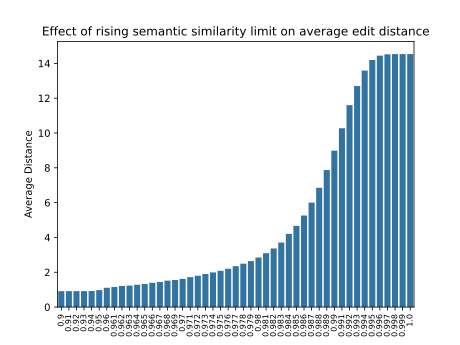
\includegraphics[width=\linewidth]{code/img/similaritylimits.pdf}
\caption{The average distance between the 38 experimental ATs per semantic similarity limit}
\label{img:similaritylimits}
\end{figure}

\NS{Operations plot}


\section{Effect of node flipping}

\NS{plot showing average distance between 38 ATs with and without node flipping}


\section{Discussion}
\label{sec:dicsussion}

% RQ1 How can we best calculate the distance between two attack trees?
% RQ2 Are these methods of attack tree distance valid?
% RQ3 What are the industry applications of attack tree distance?

\subsection{RQ1: Best Measure}

We have described five different measures of comparison between attack trees. As we see in Table~\ref{tab:counterexamples}, none of our distance measures exactly match the intuitive distance. We can confidently say that establishing distance based on underlying multiset semantics (multiset distance) and establishing distance based on a comparison of various measures is inadequate as an effective means of distance. This is further seen in Table~\ref{tab:requirmeent-suitability}, where statistical comparison and multiset distance only fully meet 3 and 5 of the 9 requirements, respectively.

Most promising are the established tree edit distance (TED) and newly developed radical distance (RD). TED is a well-established measure of distance between trees, and as such, it is not surprising that it meets almost all requirements. The only requirement it does not meet is the ability to ignore difference caused by the order of children being changed. This is seen explicitly in Table~\ref{tab:counterexamples}. TED on unordered trees is an active area of research, and as we described in Section~\ref{sec:related-work}, much of the research into unordered TED relies on exact equivalence between nodes. This is not practical for attack trees, as the labels of nodes are not identical, but should still be considered equivalent. Further research will be needed to establish unordered TED using semantic similarity between node labels to define node equivalence. Overall, TED meets 8 of our 9 requirements.

Similar to TED is our novel measure of RD. RD's allows Overall, RD fully meets 8 of our 9 requirements; for the remaining requirement of node position, RD partially meets this requirement, as it takes into account the position of nodes w.r.t. their parents but does not consider the position of the radical to the tree as a whole. When compared to our defined counterexamples in Table~\ref{tab:counterexamples}, RD matches the intuitive distance for nearly all examples. RD only does not meet expectation when the number of radicals between two trees differs.

\begin{table*}[ht!]
    \resizebox{.9\linewidth}{!}{%
    \begin{tabular}{@{}lccccccccc@{}}
                \toprule
    \shortstack{\textbf{Distance}\\\textbf{Measure}} & \shortstack{\req{1}\\\textbf{Simple}} & \shortstack{\req{2}\\\textbf{Unfiltered}} & \shortstack{\req{3}\\\textbf{Effect Size}} & \shortstack{\req{4}\\\textbf{Description}} & \shortstack{\req{5}\\\textbf{Unordered}} & \shortstack{\req{6}\\\textbf{Labels}} & \shortstack{\req{6}\\\textbf{Refinements}} & \shortstack{\req{6}\\\textbf{Position}} & \shortstack{\req{7}\\\textbf{Metric}} \\ \midrule
    \textbf{Statistics}       & \Negate                & \Confirm\footnotemark[1]          & \Negate \footnotemark[2]        & \Confirm          &\Confirm   & \Negate                 & \Confirm           & \Negate                   & \Negate\footnotemark[2]                    \\
    \textbf{TED}              & \Confirm      & \Confirm          & \Confirm           & \Confirm          & \Negate & \Confirm      & \Confirm           & \Confirm        & \Confirm      \\
    \textbf{LD}               & \Confirm      & \Confirm          & \Confirm           & \Partial \footnotemark[3]                    &\Confirm   & \Confirm      & \Negate                      & \Negate                   & \Confirm      \\
    \textbf{RD}               & \Confirm      & \Confirm          & \Confirm           & \Confirm          &\Confirm   & \Confirm      & \Confirm           & \Partial \footnotemark[4]     & \Confirm      \\
    \textbf{MSD}              & \Confirm      & \Confirm          & \Negate\footnotemark[5]                       &  \Partial  \footnotemark[3]                  &\Confirm   & \Confirm      & \Negate                      & \Negate                   & \Confirm                 \\ \bottomrule
            \end{tabular}
    }
    \caption{A comparison of the different distance measures and their suitability w.r.t. the requirements defined in Section~\ref{ssec:requirements}\\
        \footnotesize
        1: As the statistic measure does not examine labels, it is equivalently applicable to unfiltered trees.\\
        2: Without a simple definition of distance (requirement 1), this requirement is functionally impossible to meet\\
        3: These measures exclude significant information, as such their edit descriptions do not offer fully suitable descriptions of difference.\\% This requirement is partially met.\\
        4: Radical distance incorporates the position of nodes w.r.t. their parent, however, it does not incorporate the position of the radical within the whole attack tree. \\ %This requirement is partially met.
        5: Multiset distance only measures the leaf nodes, which is unable to consider the magnitude of the distance between two trees.
        \normalsize}
    \label{tab:requirmeent-suitability}
    \end{table*}

\subsection{RQ2: Validity}

To start, we apply tree edit distance, which is a well established and documented mechanism to describe the distance between two trees~\cite{Zhang_Shasha_1989,zhang_editing_1992,akutsu_tree_2021,pawlik_rted_2011,mcvicar_sumoted_2016}. If we can show the distance measures we suggest, label distance, radical distance, and multiset distance, behave similarly to tree edit distance, we can infer that these distance measures are similarly valid. In Figure~\ref{fig:semsim-at2}, we see distance measures for all distance measures as applied to a dataset of trees that all have the same base tree, but have been extended differently by participants. This distance is averaged across all samples we have, and modified by a changing semantic similarity limit. This figure shows how different distance measures change with different semantic similarity limits. This gives us a mechanism to compare different distance measures, as if measures are fundamentally measuring trees similarly, then these lines should roughly correspond to each other. We can see in Figure~\ref{fig:semsim-at2} that the tree edit distance, radical distance and label distance are all remarkably similar, with the lines for these distances translated vertically on the $y$-axis. This suggests that these distance measures are fundamentally measuring the same thing, and as tree edit distance can be argued to be valid, similarly, both label and radical distance must likewise be valid.

Figure~\ref{fig:semsim-at1-2}

Our main contribution to tree distance is the novel technique of comparing components in DAGs by using semantic similarity. To our knowledge, all previous tree distance measurements have worked with either artificial data or with a ``clean'' dataset, which would entirely negate the need to assess node similarity by anything other than equivalence. We are the first to attempt to define tree distance for node labels that are not identical, but should still be considered equivalent. By applying this method to a series of attack trees that should be more or less equivalent, we can assess if this technique is valid. As described in Section~\NS{TODO: Add section reference}, the first attack tree that subjects drew was based on a provided written scenario. Subjects were instructed to include only information provided by the scenario, to include no additional information and to include all the information in the scenario. As such and as discussed in Section~\NS{TODO: Add section reference}, while we expect natural variations in these trees due to participants interpreting the scenario differently, missing information or organizing information different, ultimately the resulting trees should be fairly equivalent. As shown in Figure~\ref{fig:semsim-at1}, for semantic similarity limits  below 0.75, we see this expected equivalence. This suggests that our method is producing an output that is measuring the distance between two attack trees, and thus is valid.

To further validate our approach, we apply our distance measurements



We have shown that our method is able to calculate the distance between two attack trees, and that this distance is valid. We have also shown that this method can be used to compare attack trees in a real-world scenario, and that it can be used to identify similar attack trees.
 

% Please add the following required packages to your document preamble:
% \usepackage{booktabs}



\subsection{RQ3: Industry Applications}



\subsubsection{Sharing Threat Intelligence}

Threat models are a recommended tool for threat analysis~\cite{andersonSecurityEngineeringGuide2020,schneierSecretsLiesDigital2000}. However, once these models are created, they may only be applicable to the analyst or the team of analysts that created them. Unlike other sources of threat intelligence, such as YARA Rules~\cite{naik2019cyberthreat,naik2020evaluating}, there is no means to share attack trees in this format.

In order to allow for attack trees to be shared as threat intelligence, two aspects are needed: a common structure and a means of comparison. The common structure has already been defined, in the ADTool XML Schema~\cite{kordy_adtool_2013}. This is an XML format used by ADTool, a tool to create Attack-Defense Trees, an extension of ATs. The ADTool XML Schema can be used to define attack trees, and as such, can be used as a common structure for sharing attack trees. The dataset of ATs we describe in Section~\ref{sec:results} is in this format. The second aspect is a means of comparison, which is what we have defined in this paper. It will be possible to publish attack trees in the ADTool XML Schema, and then compare the resulting trees using the distance measures we have defined. This will allow for the sharing of attack trees as threat intelligence, and the comparison of these trees to identify similar threats.

\subsubsection{Generative AI}

Applying generative AI to security is an active area of research. Distance measures are critical for using generative AI to create threat models in general, and attack trees specifically. By using a distance measure, we can compare the output of a generative AI to a set of known attack trees, and determine how similar the output is to the known attack trees. As we can control the form of the output of generative AI, we can have an AI tool output AT in the ADTool XML Schema, and then compare the resulting attacks to our own output or to a dataset.

Going further, in order to build and refine a generative AI tool to create attack trees, we need to define a cost function~\NS{TODO: cite something}. A cost function is necessary for training a model, as this is what the model will attempt to optimize for. Fundamental to this cost function is the ability to define distance, as we can offer a way to compare a generated solution to a ``ground truth''.


\section{Conclusion and future work}
\label{sec:conclusion}

Overall, we have proposed several new approaches for defining distance between attack trees, and have offered a comprehensive comparison between those methods. To the best of our knowledge, our work is the first to examine applying the BERT model of semantic embeddings generation to tree distance; further, we are the first to examine tree distance on tree with unfiltered (neither cleaned nor generated) node labels. We have found that traditional tree edit distance applies well with our proposed alterations of semantic similarity to determine node equivalence and an added cost for altering node refinements. Additionally, our proposed distance measure of radical distance is a promising approach for finding distance between trees. We have validated these distance measures and compared them. Finally, we have proposed applications of this research for practical use.

To further this work, we would like to examine the application of semantic similarity to determine node equivalence to potential unordered tree edit distance algorithms. We would also seek to further refine the radical distance measure to better capture the case of tree distance between trees with unequal numbers of radicals. Finally, we would like to apply these distance measures to the problem of automated attack tree generation.

% \cite{*}



\bibliography{bibliography}{}
\bibliographystyle{plain}



\appendix
\section*{Appendix}

\subsection{Operations table for counterexamples}
\begin{table*}
    \resizebox{\textwidth}{!}{
        \begin{tabular}{lcccccccccccccccc}
            \toprule
            Counterexample       & \multicolumn{4}{|c|}{Label Distance} & \multicolumn{4}{|c|}{Tree Edit Distance} & \multicolumn{4}{|c|}{Radical Distance} & \multicolumn{4}{|c|}{Multiset Distance}                                                                                                 \\
                                 & Remove                               & Add                                      & Change                                 & Match                                   & Remove & Add & Change & Match & Remove & Add & Change & Match & Remove & Add & Change & Match \\
            \midrule
            Order Reversed       & 0                                    & 0                                        & 0                                      & 7                                       & 0      & 0   & 6      & 1     & 0      & 0   & 0      & 7     & 0      & 0   & 0      & 4     \\
            Refinement Switch    & 0                                    & 0                                        & 0                                      & 7                                       & 0      & 0   & 2      & 5     & 0      & 0   & 2      & 5     & 1      & 1   & 1      & 2     \\
            Extra Intermediate   & 1                                    & 0                                        & 0                                      & 7                                       & 1      & 0   & 0      & 7     & 1      & 0   & 0      & 7     & 0      & 0   & 0      & 4     \\
            Missing Intermediate & 0                                    & 1                                        & 0                                      & 6                                       & 0      & 1   & 0      & 6     & 1      & 3   & 0      & 4     & 0      & 0   & 0      & 4     \\
            Extra Leaf           & 1                                    & 0                                        & 0                                      & 7                                       & 1      & 0   & 0      & 7     & 1      & 0   & 0      & 7     & 1      & 0   & 0      & 4     \\
            Missing Leaf         & 0                                    & 1                                        & 0                                      & 6                                       & 0      & 1   & 0      & 6     & 0      & 1   & 0      & 6     & 0      & 1   & 0      & 3     \\
            Changed Root         & 0                                    & 0                                        & 1                                      & 6                                       & 0      & 0   & 1      & 6     & 0      & 0   & 1      & 6     & 0      & 0   & 0      & 4     \\
            Changed Intermediate & 0                                    & 0                                        & 1                                      & 6                                       & 0      & 0   & 1      & 6     & 0      & 0   & 1      & 6     & 0      & 0   & 0      & 4     \\
            Changed Leaf         & 0                                    & 0                                        & 1                                      & 6                                       & 0      & 0   & 1      & 6     & 0      & 0   & 1      & 6     & 0      & 0   & 1      & 3     \\
            Move Adjacent        & 0                                    & 0                                        & 0                                      & 7                                       & 1      & 1   & 0      & 6     & 1      & 1   & 0      & 6     & 1      & 2   & 0      & 2     \\
            Move Up              & 0                                    & 0                                        & 0                                      & 7                                       & 1      & 1   & 0      & 6     & 1      & 1   & 0      & 6     & 0      & 0   & 0      & 4     \\
            Move Down            & 0                                    & 0                                        & 0                                      & 7                                       & 1      & 1   & 0      & 6     & 2      & 1   & 0      & 5     & 0      & 1   & 0      & 3     \\
            \bottomrule
        \end{tabular}

    }
    \caption{Table showing the operations per counterexample and distance measure}
\end{table*}

% \appendix
% \input{content/questionnaire}

\end{document}
